%   Filename    : chapter_4.tex 
\chapter{Research Methodology}
This chapter lists and discusses the specific steps and activities that will be performed to accomplish the project. 
The discussion covers the activities from pre-proposal to Final SP Writing.

\begin{figure}[ht]
	\centering
	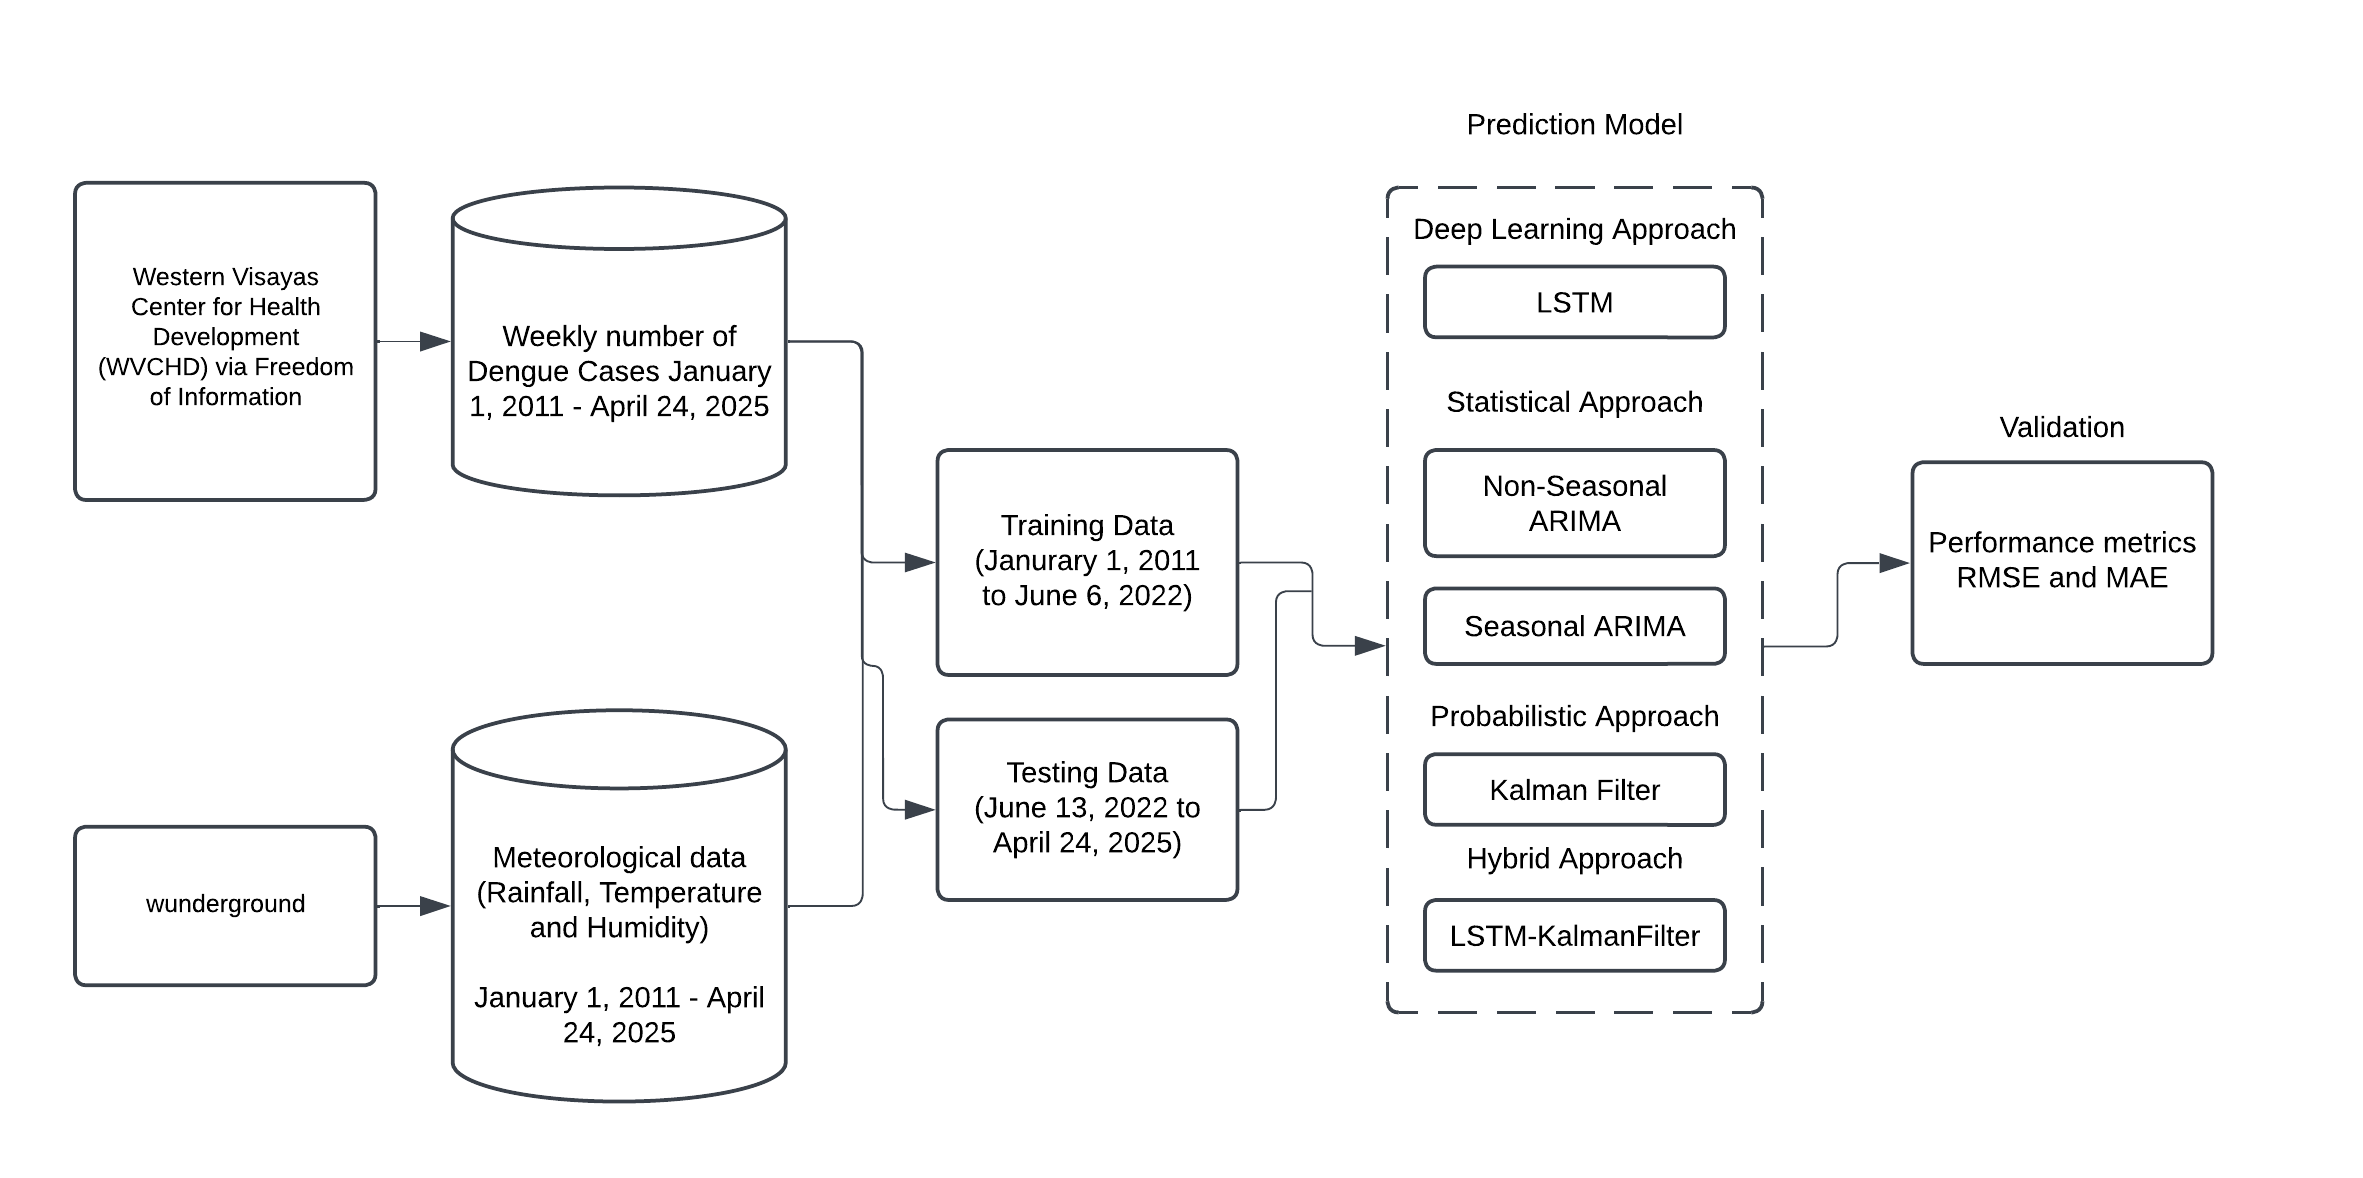
\includegraphics[width=0.75\textwidth]{Model Diagram}
	\caption{Workflow for forecasting the number of weekly dengue cases}
	\label{fig:data_snippet}
\end{figure}
This summarizes the workflow for forecasting the number of weekly dengue cases. This workflow focuses on using statistical, deep learning, and probabilistic models to forecast the number of reported dengue cases. The approach involves deploying several models for prediction, including ARIMA and Seasonal ARIMA as statistical approaches, LSTM as a deep learning approach, and the Kalman Filter as a probabilistic approach. These methods are compared with each other to determine the most accurate model.
\section{Research Activities}

\subsection{Gather Dengue Data and Climate Data to Create a Complete Dataset for Forecasting}

\subsubsection{Acquisition of Dengue Case Data}
The historical dengue case dataset used in this study was obtained from the Humanitarian Data Exchange and the Western Visayas Center for Health Development (WVCHD) via Freedom of Information (FOI) requests. The decision to use weekly intervals was driven by the need for precision and timeliness in capturing fluctuations in dengue cases and weather conditions. Dengue transmission is influenced by short-term changes in weather variables such as rainfall and temperature, which impact mosquito breeding and virus transmission cycles. A weekly granularity allowed the model to better capture these short-term trends, enabling more accurate predictions and responsive public health interventions.

Moreover, using a weekly interval provided more data points for training the models compared to a monthly format. This is particularly critical in time series modeling, where larger datasets help improve the robustness of the model and its ability to generalize to new data. Also, the collection of weather data was done by utilizing web scraping techniques to extract weekly weather data (e.g., rainfall, temperature, and humidity) from Weather Underground (wunderground.com).
\\
\\
\textbf{Data Fields}
\begin{itemize}
	\item \textbf{Time.} Represents the specific year and week corresponding to each entry in the dataset.
	\item \textbf{Rainfall.} Denotes the observed average rainfall, measured in millimeters, for a specific week.
	\item \textbf{Humidity.} Refers to the observed average relative humidity, expressed as a percentage, for a specific week.    
	\item \textbf{Max Temperature.} Represents the observed maximum temperature, measured in degrees Celsius, for a specific week.
	\item \textbf{Average Temperature.} Represents the observed average temperature, measured in degrees Celsius, for a specific week.
	\item \textbf{Min Temperature.} Represents the observed minimum temperature, measured in degrees Celsius, for a specific week.
	\item \textbf{Wind.} Represents the observed wind speed, measured in miles per hour (mph), for a specific week.
	\item \textbf{Cases.} Refers to the number of reported dengue cases during a specific week.
\end{itemize} 

\subsubsection{Data Integration and Preprocessing}
The dengue case data was integrated with the weather data to create a com
prehensive dataset, aligning the data based on corresponding timeframes. The
dataset undergoed a cleaning process to address any missing values, outliers,
and inconsistencies to ensure its accuracy and reliability. To ensure that all
features and the target variable were on the same scale, a MinMaxScaler was
applied to normalize both the input features (climate data)
and the target variable (dengue cases).

\subsubsection{Exploratory Data Analysis (EDA)}
\begin{itemize}
	\item Analyzed trends, seasonality, and correlations between dengue cases and weather factors.
	\item Created visualizations like time series plots and scatterplots to highlight relationships and patterns in the data.
\end{itemize}

\subsubsection{Outbreak Detection}
To detect outbreaks, we computed the outbreak threshold value of dengue cases using the formula, 

\begin{equation}
	\text{Outbreak Threshold Value} = \mu + 2\sigma
\end{equation}

where \(\mu\) is the historical mean and \(\sigma \) is the standard deviation.

\subsection{Develop and Evaluate Deep Learning Models for Dengue Case Forecasting}
The deep learning models were developed and trained to forecast weekly dengue cases using historical weather data (rainfall, temperature, wind, and humidity) and dengue case counts. The dataset was normalized and divided into training and testing sets, ensuring temporal continuity to avoid data leakage. The methodology for preparing and training the model are outlined below.
\subsubsection{Data Preprocessing}
The raw dataset included weekly aggregated weather variables (rainfall, temperature, wind, humidity) and dengue case counts. The "Time" column was converted to a datetime format to ensure proper temporal indexing. To standardize the data for training, MinMaxScaler was employed, normalizing the feature values and target variable to a range of 0 to 1. This step ensured that the models could efficiently process the data without being biased by feature scaling differences.

\subsubsection{LSTM Model}
The dataset was split into training and test sets to evaluate the model’s performance and generalizability:
\begin{itemize}
	\item \textbf{Training Set:} 80\% of the data (572 sequences) was used for model training, enabling the LSTM to learn underlying patterns in historical dengue case trends and their relationship with weather variables.
	\item \textbf{Test Set:} The remaining 20\% of the data (148 sequences) was reserved for testing
\end{itemize}

To prepare the data for LSTM, a sliding window approach was utilized. Sequences of weeks of normalized features were constructed as input, while the dengue case count for the subsequent week was set as the target variable. This approach ensured that the model leveraged temporal dependencies in the data for forecasting. To enhance the performance of the LSTM model in predicting dengue cases, Bayesian Optimization was employed using the Keras Tuner library. The tuning process aimed to minimize the validation loss (mean squared error) by adjusting key model hyper-parameters. The search space is summarized below:

\textbf{LSTM units:}
\begin{itemize}
	\item  min value: 32 
	\item	max value: 128
	\item	step: 16
	\item	sampling: linear
\end{itemize}
\textbf{Learning Rate:}
\begin{itemize}
	\item  min value: 0.0001 
	\item	max value: 0.01
	\item	step: None
	\item	sampling: log
\end{itemize}



The tuner was instanstiated with:
\begin{itemize}
	\item \textbf{max trials = 10:} Limiting the search to 10 different configurations
	\item \textbf{executions per trial = 3:} Running each configuration thrice to reduce variance
	\item \textbf{validation split = 0.2:} Reserving 20\% of the training data for validation
\end{itemize}

The hyperparameter tuning was conducted for three different window sizes of data: 5, 10, and 20. This allows the model to have the optimal hyperparameters used for each window size. Training was conducted over 100 epochs with early stopping to prevent overfitting while maintaining computational efficiency. A batch size of 1 was used, enabling the model to process individual sequences, which is suitable for smaller datasets but results in longer training times. The Adam optimizer, known for its adaptive learning capabilities and stability was employed.

To validate the effectiveness of the model, cross-validation was implemented. However, standard k-fold cross-validation randomly shuffles the data, which isn't suitable for time series since the order of observations is important. To address this, a time series-specific cross-validation strategy was used with TimeSeriesSplit from the scikit-learn library. This method creates multiple train-test splits where each training set expands over time and each test set follows sequentially. This approach preserves the temporal structure of the data while helping reduce overfitting by validating the model across different time segments.

After training, predictions on both the training and test datasets were rescaled to their original scale using the inverse transformation of MinMaxScaler. Model performance was evaluated using the mean squared error (MSE), root mean squared error (RMSE) and mean absolute error (MAE).

\subsubsection{ARIMA}
The ARIMA model was employed to forecast weekly dengue cases using historical weather data (rainfall, max temperature, and humidity) as exogenous variables and historical case counts as the primary dependent variable.
The dataset was split into training (80\%) and testing (20\%) sets. To determine the optimal configuration for the ARIMA model, a grid search was conducted over the following parameter ranges:
\begin{itemize}
	\item p (autoregressive order): 0 to 3
	\item d (differencing order): 0 to 2
	\item q (moving average order): 0 to 3
\end{itemize}
The combinations of these parameters were evaluated by fitting an ARIMA model for each set of (p, d, q) values. The model's performance was assessed using the mean squared error (MSE) between the predicted and actual dengue cases in the test set. The combination yielding the lowest MSE was selected as the optimal parameter configuration.

The fitted ARIMA model was used to forecast weekly dengue cases for the test dataset. Predictions were directly assigned to the PredictedCases column in the test dataset.

\subsubsection{Steps to Create the ARIMA Model:}
\begin{enumerate}
	\item \textbf{Data Preprocessing:}Prepare the dataset by handling any missing values and scaling the data if necessary to improve model convergence and stability.

\item \textbf{Hyperparameter Tuning:}  
Use a grid search on potential ARIMA parameters $(p, d, q)$ to identify the configuration that minimizes error. The optimal parameters were found to be \textbf{(1, 2, 2)}.

\item \textbf{Model Training:}
\begin{itemize}
	\item Set the number of iterations to 400 to ensure thorough training and convergence.
	\item Train the ARIMA model on 80\% of the data and reserve 20\% for testing.
\end{itemize}
\end{enumerate}


\subsubsection{Seasonal ARIMA (SARIMA)}

\begin{enumerate}
	\item \textbf{Data Preprocessing}  
	\begin{itemize}
		\item Handle missing values through interpolation or imputation.
		\item Normalize or standardize features to ensure stable training.
		\item Split data into training (80\%) and testing (20\%) sets while maintaining temporal continuity.
	\end{itemize}
	
	\item \textbf{Seasonality Analysis}  
	\begin{itemize}
		\item Perform time series decomposition to examine trend, seasonality, and residual components.
		\item Identify seasonality using autocorrelation plots and spectral analysis.
		\item A periodicity of \textbf{52 weeks} was detected, justifying the use of a seasonal model.
	\end{itemize}
	
	\item \textbf{Hyperparameter Tuning}  
	\begin{itemize}
		\item Conduct a grid search to optimize SARIMA parameters $(p, d, q)(P, D, Q)[S]$.
		\item Determine optimal configuration for seasonal and non-seasonal components.
		\item Verify stationarity through Augmented Dickey-Fuller (ADF) test.
	\end{itemize}
	
	\item \textbf{Model Training}  
	\begin{itemize}
		\item Fit the SARIMA model on the training dataset, incorporating exogenous variables such as rainfall, temperature, and humidity.
		\item Set a maximum number of iterations to ensure convergence.
		\item Monitor model diagnostics (residual analysis) to confirm the absence of autocorrelation in residuals.
	\end{itemize}
	
	\item \textbf{Forecasting and Validation}  
	\begin{itemize}
		\item Generate out-of-sample forecasts for future dengue cases.
		\item Compare predicted values against actual data to assess real-world applicability.
		\item Visualize results with line plots and confidence intervals.
	\end{itemize}
	
\end{enumerate}

\subsubsection{Kalman Filter:}
\begin{itemize}
	\item Input Variables: The target variable (Cases) was modeled using three regressors: rainfall, max temperature, and humidity.
	\item Training and Testing Split: The dataset was split into 80\% training and 20\% testing to evaluate model performance.
	\item Observation Matrix: The Kalman Filter requires an observation matrix, which was constructed by adding an intercept (column of ones) to the regressors.
\end{itemize}

The Kalman Filter's EM method was employed for training, iteratively estimating model parameters over 10 iterations. The smooth method was used to compute the smoothed state estimates for the training data. Observation matrices for the test data were constructed similarly, ensuring compatibility with the trained model.



\subsubsection{Kalman Filter Methodology with Matrix Calculations}

\textbf{Measurement Acquisition}: Obtain the measurement:
$(z_k)$ of the system's state with associated confidence. This measurement matrix provides a noisy observation of the true state.

The dataset was split into training and test sets to evaluate the Kalman Filter's performance and generalizability:
\begin{itemize}
	\item \textbf{Training Set}: 80\% of the data was used for training, enabling the Kalman Filter model to capture key patterns.
	\item \textbf{Test Set}: The remaining 20\% of the data was reserved for testing.
\end{itemize}

\textbf{Prediction Step}:
\begin{itemize}
	\item Predict the next state:
	\[
	\hat{x}_{k|k-1} = A \hat{x}_{k-1|k-1} + B u_k
	\]
	
	\item Update the state covariance:
	\[
	P_{k|k-1} = A P_{k-1|k-1} A^T + Q
	\]
	where \( Q \) is the process noise covariance matrix.
\end{itemize}

\textbf{Compute Residual}: Calculate the residual:
\[
y_k = z_k - H \hat{x}_{k|k-1}
\]
where \( H \) is the observation matrix. This residual represents the new information from the measurement.

\textbf{Scaling Factor (Kalman Gain)}:
\begin{itemize}
	\item Compute the Kalman Gain:
	\[
	K_k = P_{k|k-1} H^T \left( H P_{k|k-1} H^T + R \right)^{-1}
	\]
	where \( R \) is the measurement noise covariance matrix.
	
	\item The Kalman Gain determines the weight of the measurement relative to the prediction.
\end{itemize}

\textbf{State Update}:
\begin{itemize}
	\item Update the state estimate:
	\[
	\hat{x}_{k|k} = \hat{x}_{k|k-1} + K_k y_k
	\]
	blending the prediction and measurement.
\end{itemize}

\textbf{Uncertainty Update}:
\begin{itemize}
	\item Update the state covariance:
	\[
	P_{k|k} = (I - K_k H) P_{k|k-1}
	\]
	where \( I \) is the identity matrix.
\end{itemize}

\subsection{Integrate the Predictive Model into a Web-Based Data Analytics Dashboard}

\subsubsection{Dashboard Design and Development}
\begin{itemize}
	\item Design an intuitive, user-friendly web-based dashboard incorporating:
	\begin{itemize}
		\item Interactive visualizations of yearly dengue case trends.
		\item Data input and update forms for dengue and weather data.
		\item Map display of dengue cases in each district in Iloilo City
	\end{itemize}
\end{itemize}

\subsubsection{Model Integration and Deployment}
\begin{itemize}
	\item Deploy the best-performing model within the dashboard as a backend service to enable real-time or periodic forecasting.
\end{itemize}


\subsection{System Development Framework}
The Agile Model is the birthchild of both iterative and incremental approaches in Software Engineering. It aims to be flexible and effective at the same time by being adaptable to change. It's also important to note that small teams looking to construct and develop projects quickly can benefit from this kind of methodology. As the Agile Method focuses on continuous testing, quality assurance is a guarantee since bugs and errors are quickly identified and patched. 

\subsection{Design, Building, Testing, and Integration}
\subsubsection{Design and Developlment}
After brainstorming and researching the most appropriate type of application to accommodate both the prospected users and the proposed solutions, the team has decided to proceed with a web application. Given the time constraints and available resources, it has been decided that the said means is the most pragmatic and practical move. The next step is to select modern and stable frameworks that align with the fundamental ideas learned by the developers in the university. The template obtained from WVCHD and Iloilo Provincial Epidemiology and Surveillance Unit was meticulously analyzed to create use cases and develop a preliminary well-structured database that adheres to the requirements needed to produce a quality application. The said use cases serve as the basis of general features. Part by part, these are converted into code, and with the help of selected libraries and packages, it resulted in the desired outcome that may still modified and extended to achieve scalability. 

\subsubsection{Testing and Integration}
Each feature was user-tested to ensure quality assurance, with particular emphasis on prerequisite features, as development cannot progress properly if these fail. Moreover, integration between each feature serves as a pillar for a cohesive user experience. Presently, we have not been able to use performance metrics to measure the system's performance, as developing and connecting the core features is the utmost priority. 

\section{Development Tools}
\subsection{Software}

\subsubsection{Github}
GitHub is a cloud-based platform that tracks file changes using Git, an open-source version control system \cite{github-no-date}. It is used in the project to store the application's source code, manage the system's source version control, and serve as a repository for the Latex files used in the actual research.

\subsubsection{Visual Studio Code}
Visual Studio Code is a free, lightweight, and cross-platform source code editor developed by Microsoft \cite{vscode-2021}. As VS Code supports this project's programming and scripting languages, it was chosen as the primary source code editor.

\subsubsection{Django}
Django is a free and open-sourced Python-based web framework that offers an abstraction to develop and maintain a secure web application. As this research aims to create a well-developed and maintainable application, it is in the best interest to follow an architectural pattern that developers and contributors in the future can understand. Since Django adheres to Model-View-Template (MVT) that promotes a clean codebase by separating data models, business logic, and presentation layers, it became the primary candidate for the application's backbone. 


\subsubsection{Next.js}
A report by Statista (2024) claims that React is the most popular front-end framework among web developers. However, React has limitations that can be a nuisance in rapid software development, which includes routing and performance optimizations. This is where Next.js comes in—a framework built on top of React. It offers solutions for React's deficiency, making it a rising star in the framework race. 

\subsubsection{Postman}
As the application heavily relies on the Application Programming Interface (API) being thrown by the backend, it is a must to use a development tool that facilitates the development and testing of the API. Postman is a freemium API platform that offers a user-friendly interface to create and manage API requests \cite{postman-no-date}. 

\subsection{Hardware}
The web application is continuously being developed on laptop computers with minimum specifications of an 11th-generation Intel i5 CPU and 16 gigabytes of RAM.

\subsection{Packages}

\subsubsection{Django REST Framework}
Django Rest Framework (DRF) is a third-party package for Django that provides a comprehensive suite of features to simplify the development of robust and scalable Web APIs \cite{christie-no-date}. These services include Serialization, Authentication and Permissions, Viewsets and Routers, and a Browsable API . 

\subsubsection{Leaflet}
One of the features of the web application is the ability to map the number of cases using a Choropleth Map. Leaflet is the only free, open-sourced, and most importantly, stable JavaScript package that can do the job. With its ultra-lightweight size, it offers a comprehensive set of features that does not trade off performance and usability \cite{leaflet-no-date}. 

\subsubsection{Chart.js}
Another feature of the application is to provide users with informative, approachable data storytelling that is easy for everyone to understand. The transformation of pure data points and statistics into figures such as charts is a big factor. Thus, there is a need for a package that can handle this feature without compromising the performance of the application. Chart.js is a free and open-source JavaScript package that is made to meet this criteria as it supports various types of charts \cite{chartjs-no-date}. 

\subsubsection{Tailwind CSS}
Using plain CSS in production-quality applications can be counterproductive. Therefore, CSS frameworks were developed to promote consistency and accelerate the rapid development of web applications \cite{joel-2021}. One of these is Tailwind, which offers low-level utility classes that can be applied directly to each HTML element to create a custom design \cite{tailwind-no-date}. Given the limited timeline for this project, using this framework is a wise choice due to its stability and popularity among developers.

\subsubsection{Shadcn}
Shadcn offers a collection of open-source UI boilerplate components that can be directly copied and pasted into one's project. With the flexibility of the provided components, Shadcn allows developers to have full control over customization and styling. Since this is built on top of Tailwind CSS and Radix UI, it is supported by most modern frontend frameworks, including Next.js \cite{shadcn-no-date}.

\subsubsection{Zod}
Data validation is integral in this web application since it will handle crucial data that will be used for analytical inferences and observations. Since Zod is primarily used for validating and parsing data, it ensures proper communication between the client and the server \cite{zod-nd}. 

\clearpage
\section{Application Requirements}

\subsection{Backend Requirements}
\subsubsection{Database Structure Design}
Determining how data flows and how it would be structured is crucial in creating the system as it defines how extendible and flexible it would be for future features and updates. Thus, creating a comprehensive map of data ensures proper normalization that eliminates data redundancy and improves data integrity. Figure \ref{fig:er_diagram} depicts the designed database schema that showcases the relationship between the application's entities. 
\begin{figure}[H]
	\centering
	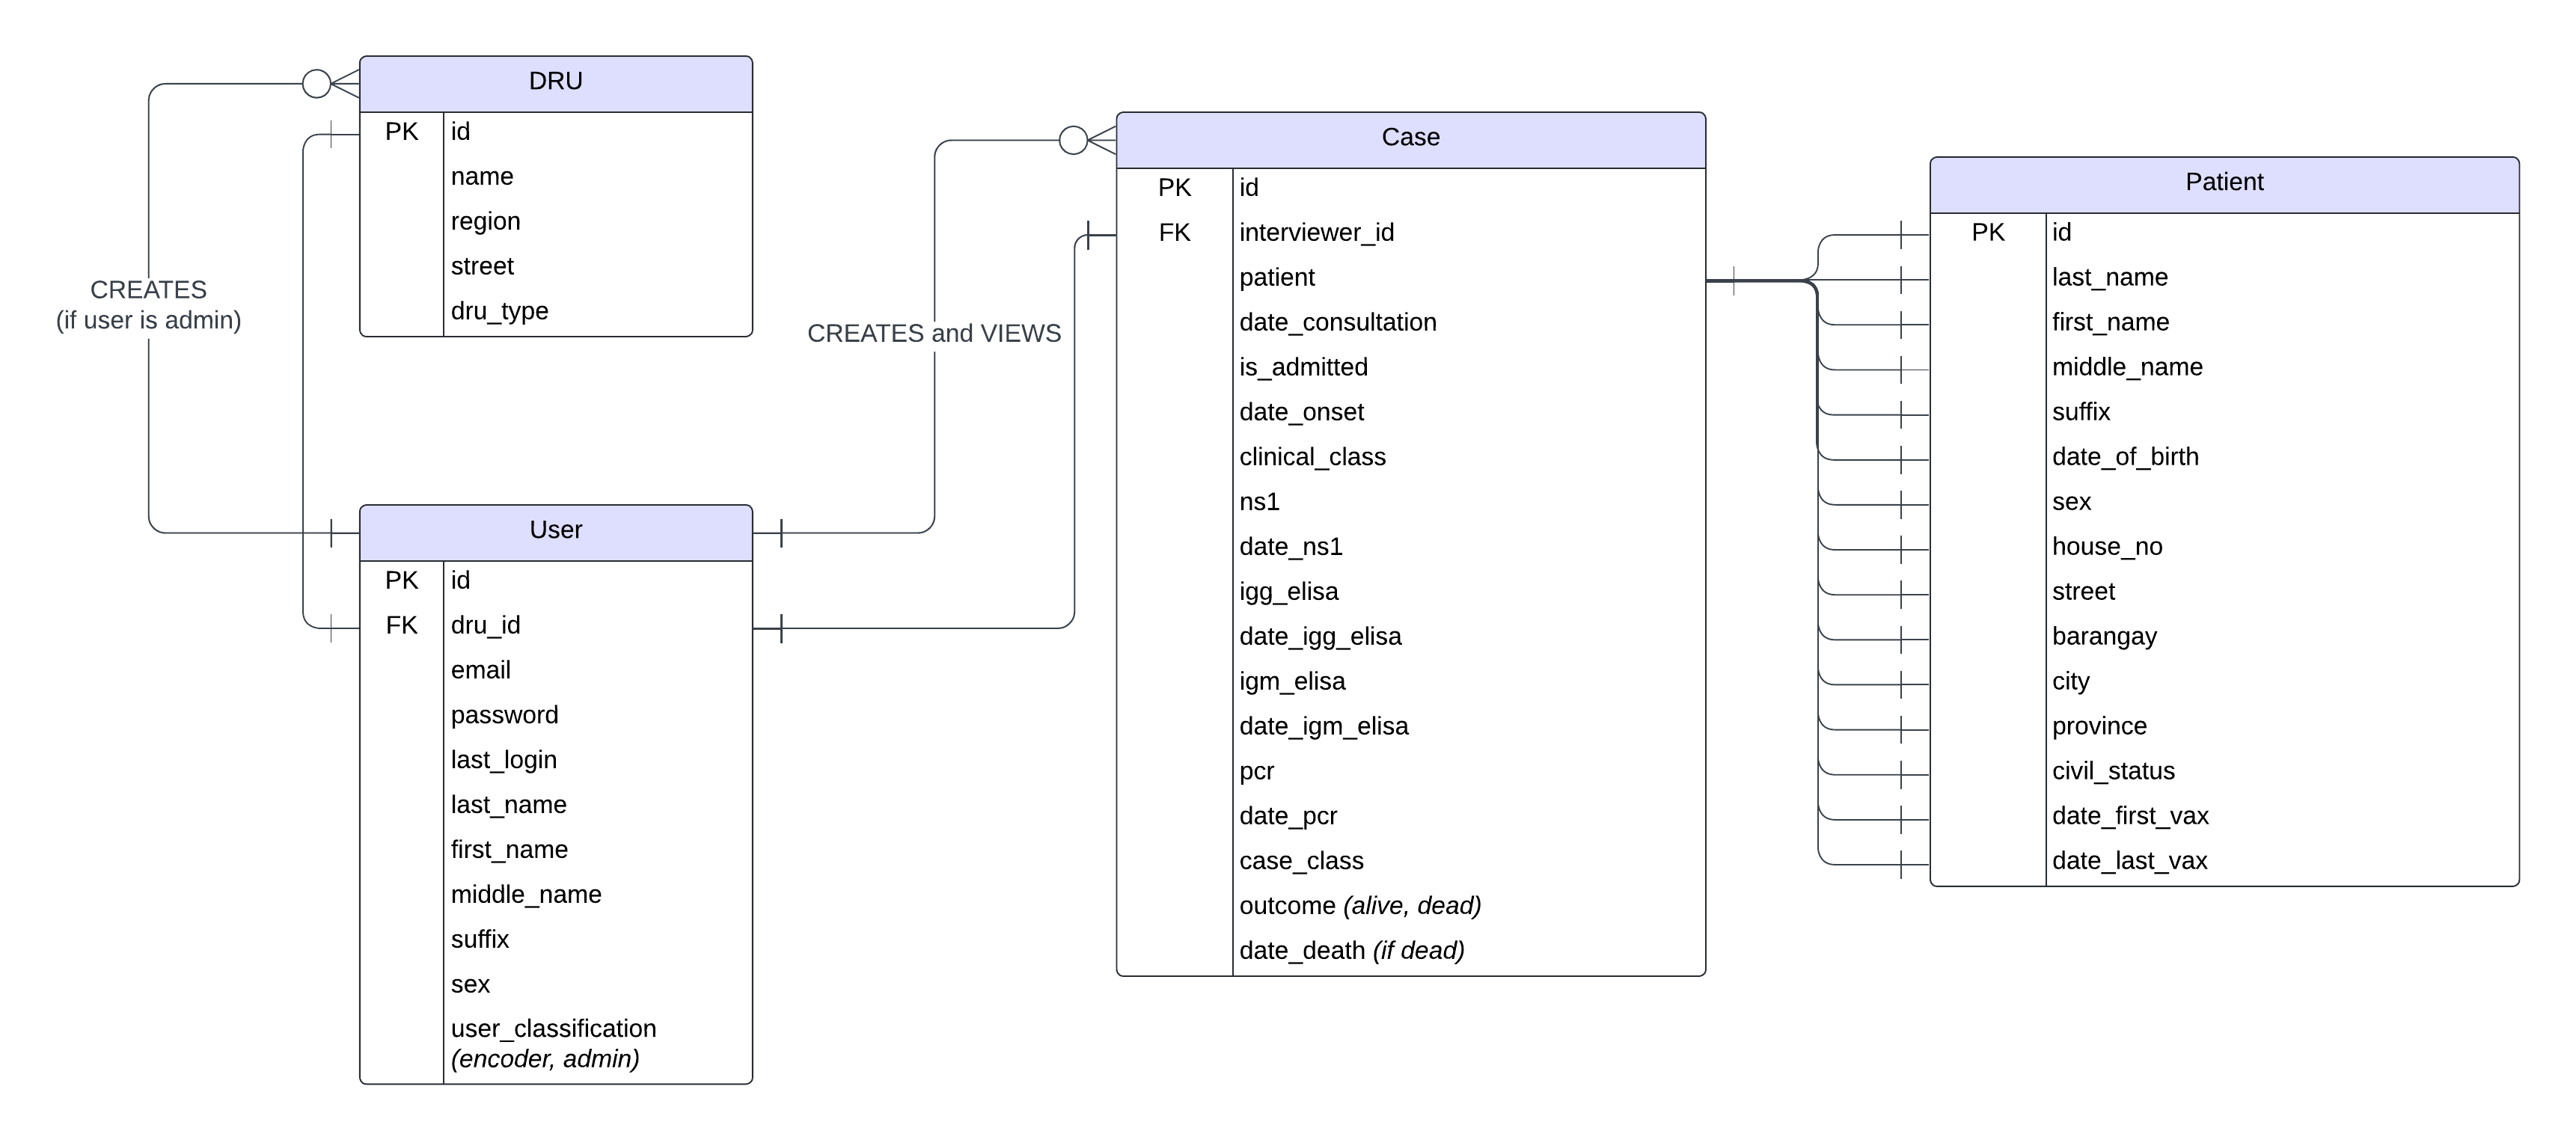
\includegraphics[width=1\textwidth]{er_diagram}
	\caption{Entity-Relationship Database Schema Hybrid Diagram for DengueDash Database Structure}
	\label{fig:er_diagram}
\end{figure}

\subsection{User Interface Requirements}
\subsubsection{Disease Reporting Unit Admin Interface}
\begin{figure}[H]
	\centering
	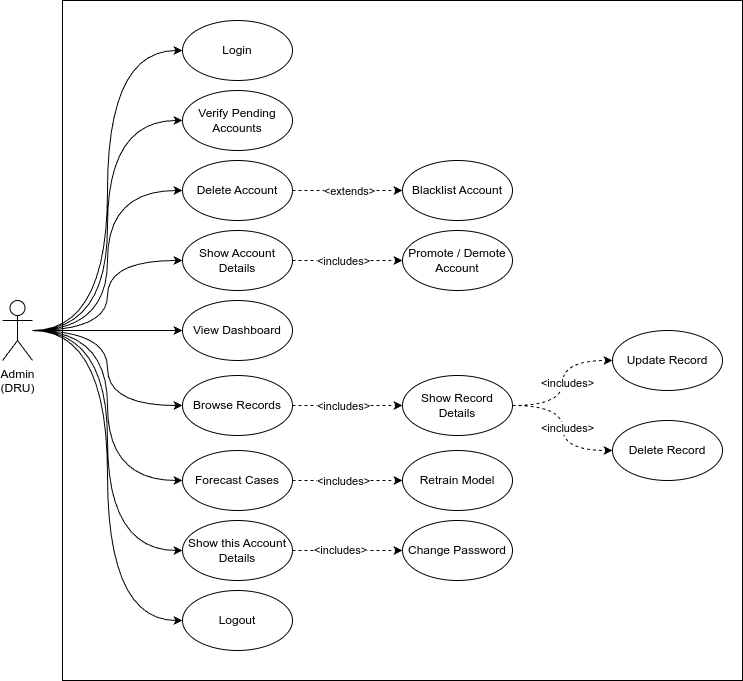
\includegraphics[width=1\textwidth]{admin_dru}
	\caption{Use Case Diagram for DRU Admin}
	\label{fig:admin-dru-use-case}
\end{figure}
\subsubsection{Surveillance Unit Admin Interface}
Figure \ref{fig:admin-dru-use-case} shows the actions an admin for a specific Disease Reporting Unit (DRU) can take in the application. These include managing accounts, browsing records, and forecasting and retraining all the consolidated data under the unit. To protect the integrity of data, encoders that register to a DRU must first be verified by these users, and then the encoder's account can only be authorized to use the application. 
\begin{figure}[H]
	\centering
	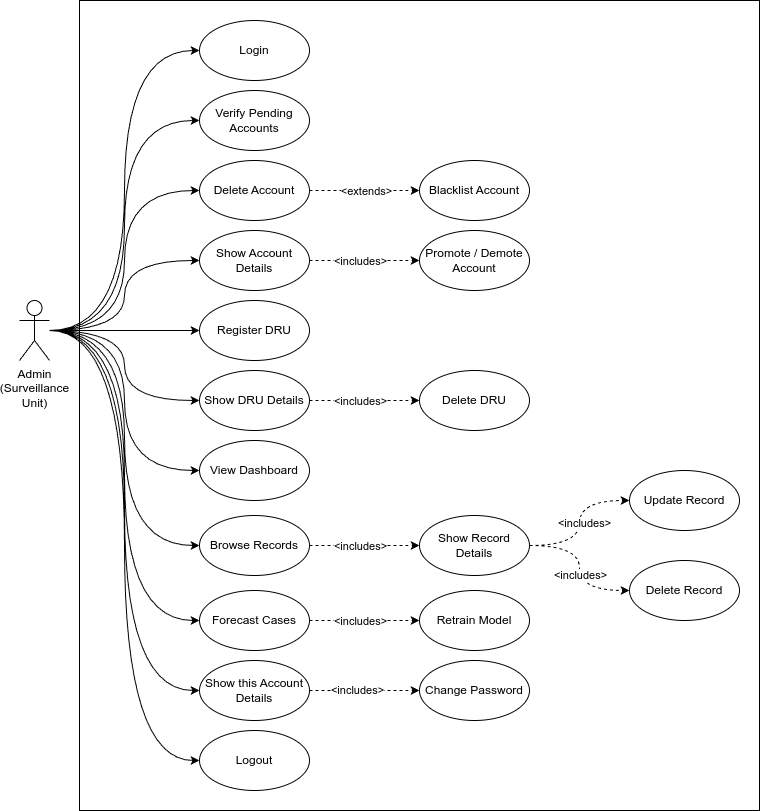
\includegraphics[width=1\textwidth]{admin_su}
	\caption{Use Case Diagram for Surveillance Unit Admin}
	\label{fig:admin-su-use-case}
\end{figure}
While the previous use case focuses on hospitals, clinics, and other reporting units, the use case presented in Figure \ref{fig:admin-su-use-case} has a one-step higher authorization as it manages these DRUs. It has the same features as the DRU admin but with extra management of the DRUs under a specific surveillance unit. At this point, only the authorized surveillance unit administrator can register and create a DRU to uphold transparency and accountability. 


\subsubsection{Encoder Interface}
\begin{figure}[H]
	\centering
	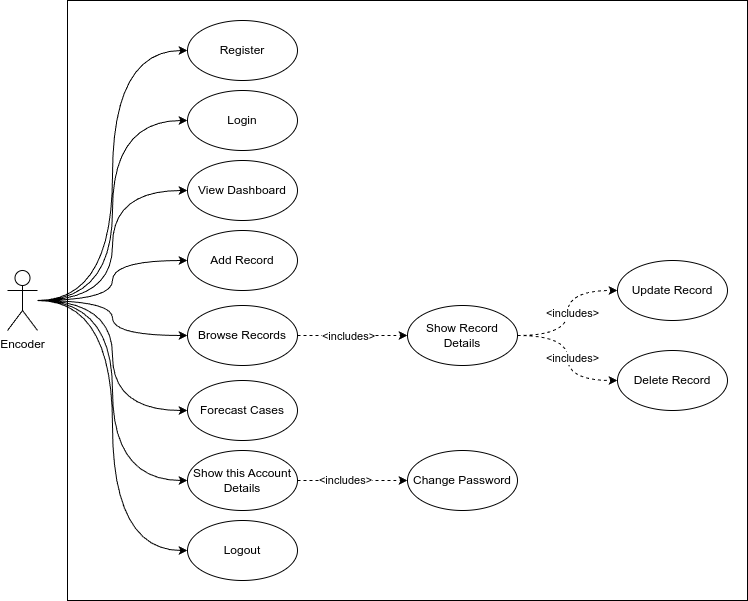
\includegraphics[width=1\textwidth]{encoder}
	\caption{Use Case Diagram for Encoder}
	\label{fig:encoder-use-case}
\end{figure}

Figure \ref{fig:encoder-use-case}, on the other hand, illustrates the use cases for the system's primary users. These users can register but must wait for further verification to access the application. Similar to the previous interfaces, encoders can browse and manage records, as well as forecast the consolidated cases under a specific surveillance or disease reporting unit, but they are not allowed to retrain the model. Lastly, they are the only type of user that can file and create dengue cases by filling out a form with the required details.


\subsection{Security and Validation Requirements}
\subsubsection{Password Encryption}
Storing passwords as plain text in the database is a disgrace and a mortal sin in production. It is important to implement precautionary methods such as hashing and salting, followed by encryption with a strong algorithm, to prevent bad actors from using the accounts for malicious transactions. By default, Django generates a unique random salt for each password and encrypts it with Password-Based Key Derivation Function 2 (PBKDF2) with a SHA256 hash function. Utilizing these techniques ensures that in the event of a data breach, cracking these passwords would be time-consuming and useless for the attackers. 

\subsubsection{Authentication}
DengueWatch utilizes JSON Web Tokens (JWT) to authenticate the user. Since the mechanism operates in a stateless manner, tokens are served only after a successful login, eliminating the need for the server to keep a record of the token, which is vulnerable to session hijacking. In addition, these tokens are signed with a secret key, ensuring they have not been tampered with. 

\subsubsection{Data Validation}
Both the backend and frontend should validate the input from the user to preserve data integrity. Thus, Zod is implemented in the latter to help catch invalid inputs from the user. By doing this, the user can only send proper requests to the server which streamlines the total workflow. On the other hand, Django has also a built-in validator that checks the data type and ensures that the input matches the expected format on the server side. These validation processes ensure that only valid and properly formatted data is accepted, which reduces the risk of errors and ensures consistency across the web application. 

\subsection{Testing Process}
\begin{figure}[H]
	\centering
	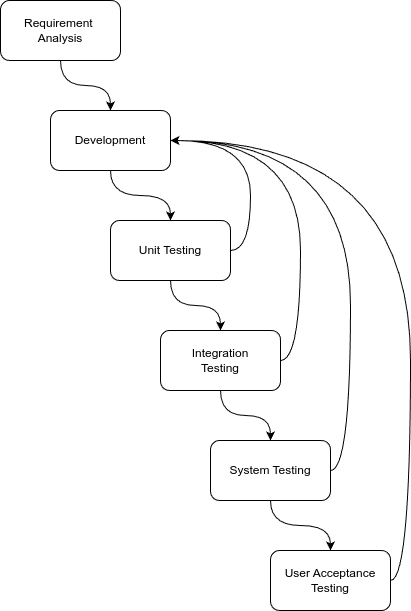
\includegraphics[height=10cm]{testing_process}
	\caption{Testing Process for DengueWatch}
	\label{fig:testing-process}
\end{figure}

As the system requirements and functionalities have been mentioned above, it is important to implement testing to validate the system's performance and efficacy. Since dengue reports include confidential information, anonymized historical dengue reports were used to train the model and create the foundational architecture of the system. By using functional tests, data validation and visualization can be ensured for further continual improvements. Security testing is also important as it is needed to safeguard confidential information when the system is deployed. It includes proper authentication, permission views, and mitigating common injection attacks. Finally, a user acceptance test from the prospected users, in this case, doctors, nurses, and other health workers, is crucial to assess its performance and user experience. It enables the developers to confirm if the system meets the needs of the problem, and once confirmed, it will be deployed and further evaluated to ensure stability and reliability in live operation. 


\section{Calendar of Activities}

A Gantt chart showing the schedule of the activities is included below. Each bullet represents approximately one week of activity.

\newcommand{\weekone}{\textbullet}
\newcommand{\weektwo}{\textbullet \textbullet}
\newcommand{\weekthree}{\textbullet \textbullet \textbullet}
\newcommand{\weekfour}{\textbullet \textbullet \textbullet \textbullet}

\begin{table}[ht]
	\centering
	\caption{Timetable of Activities for 2024} \vspace{0.25em}
	\begin{tabular}{|p{2in}|c|c|c|c|c|c|c|c|c|c|c|} \hline
		Activities & Aug & Sept & Oct & Nov & Dec \\ \hline
		Project Initiation and Team Formation & \weektwo & & & & \\ \hline
		Literature Review and Data Gathering & \weektwo & \weekfour & & & \\ \hline
		Data Cleaning and Feature Selection & & \weektwo & & \weekone & \weekone \\ \hline
		Creating System Dashboard & & \weektwo & \weekfour & \weekone & \\ \hline
		Analysis and Interpretation of Results & & & \weekone & & \weekone  \\ \hline	
		Documentation & \weektwo & \weekfour & \weekfour & \weekfour & \weekfour  \\ \hline	
	\end{tabular}
	\label{tab:timetableactivities2024}
\end{table}

\begin{table}[ht]
	\centering
	\caption{Timetable of Activities for 2025} \vspace{0.25em}
	\begin{tabular}{|p{2in}|c|c|c|c|c|c|c|c|c|c|c|} \hline
		Activities & Jan & Feb & Mar & Apr & May \\ \hline
		Create Admin Dashboard & \weekone & \weekthree & & & \\ \hline
		Integrate the Best Model to the System & \weekone & \weekfour & & & \\ \hline
		Extend Features to Accommodate a National Setting & & \weekone & \weektwo & & \\ \hline
		User Testing & & & \weektwo & \weekone & \\ \hline
		System Deployment & & & & \weekthree & \\ \hline
		Documentation & \weektwo & \weekfour & \weekfour & \weekfour & \weekfour  \\ \hline		
	\end{tabular}
	\label{tab:timetableactivities2025}
\end{table}



